\documentclass[conference]{IEEEtran}
\usepackage{fancyhdr}\usepackage[utf8]{inputenc}
\usepackage{graphicx}
\usepackage{multirow}

\usepackage{lastpage}

%\usepackage{draftwatermark}


%\SetWatermarkText{UoA}
%\SetWatermarkScale{3}

\pagestyle{fancy}
\fancyhf{}
\rfoot{Page \thepage \hspace{1pt} of \pageref{LastPage}} 

\title{Is it Possible to Extend IPv6?}
\date{December 2022}

\author{\IEEEauthorblockN{Ana Custura}
\IEEEauthorblockA{
\textit{University of Aberdeen}\\
}
\and
\IEEEauthorblockN{Raffaello Secchi}
\textit{University of Aberdeen}\\
\and
\IEEEauthorblockN{Gorry Fairhurst}
\textit{University of Aberdeen}\\
}
\begin{document}

\maketitle

\begin{abstract}
The IPv6 Hop-by-Hop Options and Destination Options Extension Headers have historically faced challenges in deployment due to the lack of support in hardware-based forwarding and concerns around potential denial-of-service attacks. However, there has been a renewed interest within the standards community both in simplifying their processing, and in using them for new applications. 
Through a wide-scale measurement campaign, we show that many autonomous systems in access networks and core of the Internet permit the traversal of EHs including Options, and that path traversal depends on the type of network, size of Option and transport protocol used, but does not depend on the type of Option included. We show that packets including Extension Headers can impact load balancing network functions, and present evidence of equipment mis-configuration. Finally, we outline the current deployment challenges  and provide recommendations for utilizing new Options to extend IPv6.

\end{abstract}

\begin{IEEEkeywords}
IPv6 protocol, Extension Headers, Protocol Evolution, Destination Options, Hop-by-hop Options
\end{IEEEkeywords}

\section{Introduction}
\label{sec:introduction}

IPv6 Extension Headers (EHs)~\cite{RFC8200} are optional headers that a source node can
add to the base IPv6 header to include extra functionality and features as a packet traverses an IPv6 network path. They were defined in the IPv6 specification
to ensure the protocol was flexible and extensible.
%The use of extension headers allows for a flexible and extensible design of IPv6 that can support a variety of new networking features and technologies.
% commented out as it does not say much
IPv6 EHs are widely used to implement specific functions. 
However, in this paper we focus on network support for two key EHs: the Destination Options (DST) header and the Hop-by-Hop Options (HBH) header~\cite{rfc9098}, as they are the primary means to extend IPv6 functions.


Recent presentations to the networking community have commented on the limited path traversal of packets including EHs and remarked that network devices, such as firewalls, routers, load balancers and intrusion detection systems~\cite{nalini-iepg114, fernando-talk} do not properly handle packets including an EH. This can result in a drop of the packet including the EH (i.e., the packet fails traverse the end-to-end network path).

Additionally, some network administrators may use firewalls to implement Access Control Lists (ACLs) at the outer edge of access and enterprise networks, which discard packets including an EH. This is done to mitigate security concerns, such as bypassing security mechanisms or defending against denial-of-service (DoS) attacks~\cite{naagas2021deh}.


Plausible reasons for limited traversal of packets including EHs are documented in~\cite{ietf-v6ops-hbh-03}, where the authors note that early IPv6 routers
processed EHs in software. This processing of EHs would normally utilise the slow-path, rather than the optimised fast-path, resulting in decreased router forwarding rates. In some designs, this processing consumed resources that would normally be used for Control Plane processing, opening up a potential DoS attack vector on the critical router functions (reducing ability to perform routing, management, etc). This motivated network operators to implement policies to drop packets that include EHs~\cite{rfc9098}.  This, in turn,
discouraged use of EHs and their successful standardisation. 

However, important recent changes motivate the need to take a fresh look at the usability of EHs as a mechanism to extend IPv6: modern high-speed routers have introduced flexible forwarding hardware that can support the ability to parse and process simple headers within the fast-path~\cite{programmable-data-plane, cisco-silicon-one, hauser2023}; and specific use-cases have emerged where there is an operational demand for new techniques that could be realised through EHs.

%XXX at some point here we will include a ref to ASIC XXX

The paper provides insight into whether these changes in operations and equipment have impacted the forwarding of packets that include the HBH and DST EHs, and seeks to understand the opportunity to use these EHs to implement new functions. It begins by discussing previous independent measurements that have reported variable results on the traversal of IPv6 packets that include an EH~\cite{RFC7872} \cite{apnic} \cite{nalini-iepg114} \cite{james}.
It then presents a broad dataset collected to explore key aspects (e.g., the size of the EH, the choice of transport, and choice and composition of the EH Options), revealing a more diverse and nuanced picture of Internet paths than was previously reported.

%XXX Unsure I think the next para is well placed, nor necesarily the correct story ... the shape of this depends on journal style XXX

Specifically, the results demonstrate that if  EHs are limited in size,
packets including a DST EH can traverse as many as
95\% of a diverse set of Internet paths. While HBH EH packets only traverse a narrow set of paths, when we
characterise whether packets traverse Autonomous Systems (AS), if we exclude operator policies in access and transit networks, we find many ASes forward packets that include this type of EH.

This paper also presents novel insights into the forwarding of packets that include a DST or HBH EH. Our research findings
demonstrate that the inclusion of some EHs in packets on paths with a form of network layer load-balancing often results in a narrower set of forwarding paths. Although one could interpret this as an alternative approach to extracting entropy from EHs, it is more likely a
pathological outcome of load balancing network routers not configured to support packets that include EHs.
We recpmmend that eliminating these pathologies would open up opportunities for
developers and network operators to take advantage of a range of recently-standardised or in-progress innovative ideas based on EHs, such as tools to monitor network performance~\cite{rfc8250}~\cite{ietf-ippm-ioam-ipv6-options-10} or enabling larger packets~\cite{rfc9268}.

%XXX Summary para below XXX

The remainder of this paper is organised as follows:  Section~\ref{sec:background} presents
the required background for IPv6 EHs and describes the historical challenges related to their deployment.  The previous literature describing measurement of paths using packets including IPv6
EHs is surveyed in Section~\ref{sec:motivation}.
Sections~\ref{sec:methodology}-\ref{sec:pathspider-results} present the
methodology and results of this study, organised by the type of network path.  The
implications of our results are discussed in Section~\ref{sec:discussion}.
Finally, the conclusion summarises our findings.

\section{Extending IPv6}
\label{sec:background}

%%XXX EH or OPT????????

\label{sec:ipv6-option-deployment}

\begin{figure}
\centering
  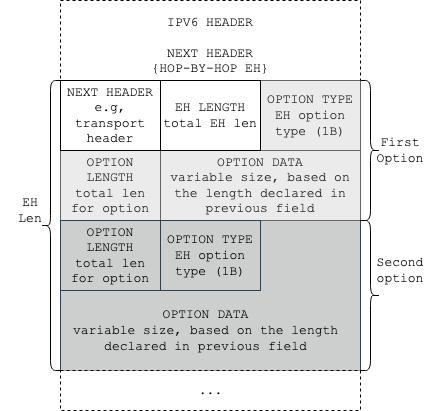
\includegraphics[width=0.5\textwidth]{ehformat.png}
  \caption{IPv6 packet with a base header that includes two EHs}
  \label{fig:eh-format}
\end{figure}


The original IPv6 specification~\cite{rfc2460} introduced a flexible header structure consisting of a fixed-length base header and one or more optional Extension Headers (EHs). 
IPv6 became a full standard in 2017~\cite{RFC8200}. This updated RFC 2460, and also changed some of the processing rules for EHs to align with the current operational practice. RFC 8200~\cite{RFC8200} allows multiple EHs in a single packet providing that they can fit the first fragment in case of fragmentation. 

The type of the first EH is denoted in the Next Header field of the IPv6 base header. Each consecutive EH contains a Next Header field to specify the type of the following EH, forming a chain terminated by the IPv6 payload. Each EH also contains a Length field specifying its total length. 

Besides HBH and DST, the types of EH include Routing, Fragment, and
Authentication and the Encapsulating Security Payload Header.
The Fragment header, Authentication and Encapsulating Security Payload header operate end-to-end and follow the Routing header if present. 

When a HBH EH is included, it must be placed immediately after the base header~\cite{RFC8200}.  The DST EH is the only EH which is permitted to be included more than once (i.e., it can appear before and after the Routing EH). 

The Routing EH is widely used by SRv6 to ensure the path includes specified intermediate nodes, typically within a single domain. SRv6 is currently deployed and actively researched~\cite{srv6}~\cite{srperf}.
Since the HBH (and first DST) come before the Routing EH, they have to be processed or skipped for routers that act as SRv6 intermediate nodes, to allow them to update the destination address using the Routing EH.

The final place a DST EH can appear is directly before the payload and is meant to be consumed at the final destination endpoint. This is propagated transparently over a network path. The DST and HBH EHs are the primary means by which IPv6 functions can be extended, by defining new Options.


Options use a Type-Length-Value (TLV) encoding~\cite{RFC8200} with 1~byte for each of the Type and Length fields, and a variable-sized Value field that carries the Option data. Their total length is always a multiple of 8 bytes to preserve alignment. Figure~\ref{fig:eh-format} shows the structure of an IPv6 packet including a base header followed by a HBH EH containing two Options.


A router can skip any Options that it does not understand. In addition, when an Option is unknown, the two most significant bits of the Type
specify the action a router should take to address the unrecognised header. When the two most significant bits are 00, the router should
ignore the Option and continue processing the header. If these bits are 01, the
processing should stop and discard the packet. If the bits are 10,
the packet should be discarded and an ICMP notification should be returned to
the sender. Finally, if the bits are 11, the same actions as for 10 should occur,
but this notification should be sent only if the destination address was not multicast. 

Table~\ref{tbl:options} presents the currently standardised 
Options.  We observe that most Options set the two most significant bits
(MSBs) to 00.  The third most significant bit specifies, if set, that the Option data field can be modified en route.

Because HBH Options can be modified by routers on a path, they can be used to provide and collect data from routers to support measurement. This has opened up opportunities for innovative alternatives to traditional mechanisms for measurement (e.g., using ICMP): Option 0x30 provides additional input to inform  PMTUD or PLPMTUD~\cite{rfc9268}, Option 0x12 has been specified to measure packet loss, latency, and jitter on live traffic measurement~\cite{rfc9343} and recently-proposed Option 0x31 records operational and telemetry information that can be updated by routers on then path between two endpoints.
Originally, all routers on a path were required to examine and process the HBH EH~\cite{rfc2460}. This requirement was realxed by~\cite{RFC8200} to only require processing when support is  configured.


DST can carry Options that provide similar functionality. Option 0x0F~\cite{rfc8250} can be used to measure performance and provide diagnostic metrics such as round-trip delay. 


% The total EH length is 8-byte aligned and specified in the
% EH Length field, while each individual option declares its own length in the
% Option Length field. 

\begin{table}[b]
\center
\caption{Currently Standardised DST and HBH Options.}
\begin{tabular}{p{0.03\textwidth}|p{0.055\textwidth}|l|p{0.18\textwidth}}
Hex  & MSBs & Type      & Description                                              \\
\hline
\hline
0x00 & 000  & HBH, Dest & Pad1 (padding)                                           \\
0x01 & 000  & HBH, Dest & PadN (padding)                                           \\
0xC2 & 110  & HBH       & Enable jumbo payloads                                    \\
0x23 & 001  & HBH       & Low-Power and Lossy Networks routing                     \\
0x04 & 000  & Dest      & Mechanism for IPv6 encapsulation                 \\
0x05 & 000  & HBH       & Mechanism for requesting router processing, Router Alert              \\
0xC9 & 110  & Dest      & Mobility Support in IPv6                                 \\
0x8C & 100  & Dest      & Method for identifying subscribers in broadband networks \\
0x6D & 011  & HBH       & Multicast Protocol for Low-Power and  Lossy Networks     \\
0x0F & 000  & Dest      & Delay measurement                                        \\
0x30 & 001  & HBH       & PathMTU                                     \\
0x11 & 000  & HBH, Dest & \multirow{2}{*}{On-path operational info}                \\
0x31 & 001  & HBH, Dest &                                                          \\
0x12 & 000  & HBH, Dest & On-path telemetry                                       
\end{tabular}
  \label{tbl:options}
\end{table}


\subsection{Previous Studies of IPv6 EHs}

\label{sec:motivation}

The debate on whether or not IPv6 packets that include EHs traverse the Internet is not new to the Internet community.
In 2015, an Informational IETF document presenting traceroute active
measurements to destinations within the Alexa top 1M domains~\cite{RFC7872}
revealed that packets including EHs experience a significantly higher drop rate over an
Internet path compared to packets that do not include EHs. Since then, other
studies~\cite{james}~\cite{nalini-iepg114}~\cite{apnic} have appeared within the standards community that support this claim.  However,
the level and nature of the reported loss varied significantly in these
reports.  This suggests the need for more analysis into the causes of loss and the need to define new measurement methods~\cite{james}~\cite{elkins-v6ops-eh-deepdive-fw-01}.  


Another IETF draft, ``Just Another Measurement of Extension header
Survivability" (JAMES)~\cite{james}, presents results for EH path traversal using
traceroute measurements over a mesh network with 21 vantage points located in a set of globally distributed Autonomous Systems (ASes). This study tests all the standard EHs
(including Routing, Fragment, etc.) in a setting where both ends of the
communication path are under the control of the researcher.  It reported traversal in only 8-9\% of paths for an 8 Byte (B) HBH, and a 97\% traversal for an 8~B DST. The traversal decreases as the size of the EH
increases~\cite{james-imc}. We note 6 of the 21 vantage points were
hosted by Digital Ocean\texttrademark, a cloud provider which drops packets including the HBH EH.

An innovative measurement methodology was built to analyse end-to-end path traversal
rates for Fragmentation, HBH and DST by engineers in APNIC~\cite{apnic}.  This technique initiates TCP connections from clients using a crowd-sourced approach. It performs  end-to-end measurements by replying to requests with packets that include an EH. If a client then replies to the packet including the EH, the test is considered successful.  
APNIC has reported results from 4M measurements/day from clients across the IPv6 Internet.  Their findings show that 50\%  of clients reply where DST is included and close to zero where HBH is included.
However, we note that this test does not simply measure traversal over an Internet path, but also whether or not endpoint nodes reply to a packet that includes an Option. 
%We also note that all measurements were performed from servers in a
%single Cloud provider (Linode).

% The different results outlined above present conflicting views, representative
% of the complex nature of Internet paths. We argue the differences are explained
% by examining the types of networks measured and the choice of vantage points
% and destinations. To fully explore the various aspects of EH traversal, our
% work takes a large-scale measurement approach, testing a wide range of access,
% core and server edge networks, and focuses on the HBH and DST EH types.
% In Section~\ref{sec:discussion}, our results from measurements in access
% networks are compared and discussed alongside their closest counterpart - the
% measurements presented in JAMES~\cite{james}. As we also test edge paths to
% target servers based on top 1M domains lists, we refresh the data presented
% in~\cite{RFC7872} for a longitudinal view.

A large passive measurement campaign used the Czech Republic national
research and education network to analyse IPv6 traffic over a period of one month in
2016~\cite{passive-threats}. It found that 0.1\% of IPv6 flows
that include an EH, out of which 40.9\% were packets including HBH with an ICMPv6
payload, primarily multicast (although not specified by the original authors,
we identify this as Multicast for Low-Power and Lossy Networks~\cite{RFC7731}).
The study noted that dropping ICMPv6 traffic that include EHs could result in
loss of essential network control information. 

% With the exception of~\cite{james-imc}, there are no other peer-reviewed active
% measurement studies. 

Our large-scale measurement study complements the previous analyses. It not only
looks at the end-to-end support in servers, but also provides comparative path
analysis and longitudinal changes in the traversal for HBH and DST.

\subsection{Challenges and Operational Considerations}

The parsing of IPv6 packets that include an EH depends on 
the router implementation and architecture. There are different types of router designs on the end-to-end path, from Customer Premises Equipment (CPE) access network routers to high-speed routers within transit networks that can handle thousands of GB/s. As the Internet became widespread, many high-speed routers have adopted a split architecture, 
with a forwarding plane~\cite{RFC3654}, often utilising hardware support, and a control plane, implemented in software (also used for router-critical operations used to manage and control the router)~\cite{router-architecture}.
In some architectures, incoming packets can be processed on the ``fast-path" in the forwarding plane on an Application Specific Integrated Circuits (ASIC) or processed on the ``slow-path" in software, possibly using the control plane processor~\cite{RFC3654}.

As IPv6 emerged, router architectures that process all packets that include EHs using the control plane were designed~\cite{ietf-v6ops-hbh-03}.  This resulted in exposing these routers to DoS attacks~\cite{naagas2021deh}, by sending a large amount of IPv6 traffic including EHs to target their control plane functions where no mitigation was available (e.g. by reducing the rate of packets, or rate-limiting). This, in turn, motivated network operators to configure their routers to discard packets that included an EH, in particular the HBH EH, which can lead to undesirable effects~\cite{passive-threats}. We show this likely remains a challenge to EH deployment.
Some routers might also discard packets including EHs due to buggy implementations~\cite{passive-threats}.

In addition, certain network nodes need to inspect the transport protocol information, for example, to inspect ports in the upper-layer protocol header for implementing an ACL or another security policy.
This requires parsing the entire IPv6 header chain, from the base header to the last EH.Such nodes are common at a network domain edge, including the edge of enterprise and home networks.

Other examples of utilising upper layer protocol headers include: Routers performing Equal Cost Multipath Routing (ECMP), application-layer load balancing, Multi-field classifiers for QoS, deep packet inspection (DPI) and DoS attack mitigation~\cite{lb-classification}. Other access-network routers can modify upper layer protocol headers to avoid issues introduced by encapsulation, e.g., by performing TCP Maximum Segment Size (MSS) Clamping~\cite{custura-mtu}.


A different set of considerations applies to routers that operate in transit networks, which typically do not require upper-layer protocol information.
RFC 9288~\cite{rfc9288}  provides recommendations for transit routers. While this recommends forwarding packets on the fast-path, or using the slow-path providing that there is a mechanism to control the  packet rate. Where no mitigation choices are present, this recommends to discard packets that include these EHs. 


%In the early Internet, packet routers were implemented entirely
%in software, and as the Internet grew packet processing was moved from software
%to Application Specific Integrated Circuits (ASICs), while the control
%functions remained~\cite{router-architecture}. Routers started having a split
%architecture with a control and forwarding plane~\cite{RFC3654}, corresponding
%to router-critical operations running in software and hardware processing
%respectively. 
%In this architecture, incoming packets can be processed on the
%``fast-path" in the forwarding plane on an ASIC or sent for processing over an
%internal link on the ``slow-path", or the control plane of a router. 

%As IPv6 emerged, ASIC support for it was limited, and IPv6 deployment itself was in its infancy - and many network router architectures processed packets containing IPv6 EHs in software~\cite{ietf-v6ops-hbh-03}.  This resulted in opening these routers up to DoS attacks~\cite{naagas2021deh}, because clients sending a large amount of IPv6 traffic including EHs could affect a router's control plane functions where no rate-limiting of such packets was available. This steered
%network operators to configure their routers to discard packets containing EHs,
%in particular the HBH EH~\cite{ietf-v6ops-hbh-03}.

%https://ieeexplore.ieee.org/stamp/stamp.jsp?tp=&arnumber=7949061

%\subsection{Hop-by-Hop and Destination Option EHs}

%An IPv6 packet can contain zero or more EHs, each identified by its own number
%in the Next Header field in the preceding header. The HBH header is
%indicated by the value 0, while the assigned protocol number for the DST
%header is 60. Both HBH and DST can be included in the same IPv6 packet in
%different EHs. An EH can contain multiple Options - Figure~\ref{fig:eh-format}
%presents one EH including 2 Options.


% Although intended to be
% processed differently, HBH and DST EHs carry a variable number of Options
% that share the same Type-Length-Value (TLV) encoding~\cite{RFC8200}. Option
% Type and Length are each encoded within one Byte, followed by a variable-size
% Option Value field that carries the option data. Figure~\ref{fig:eh-format}
% shows this format. The total EH length is 8-byte aligned and specified in the
% EH Length field, while each individual option declares its own length in the
% Option Length field. Standardized option types are presented in
% Table~\ref{tbl:options}.

% Please add the following required packages to your document preamble:



%\subsection{Operational considerations}

%\textbf{POSSIBLY MOVE THIS SECTION BELOW}



\section{Methodology} 
\label{sec:methodology}

This paper employs a combination of tools and experiments that
delve into various aspects of HBH and DST traversal. Table~\ref{tbl:datasets} presents the purpose and name of each resulting dataset, alongside the time periods for each measurement and the used transport protocol. The setup for each test is discussed in the next subsections.


\begin{table}
\begin{tabular}{p{0.17\textwidth}|p{0.075\textwidth}|p{0.03\textwidth}|p{0.065\textwidth}|p{0.03\textwidth}}
Purpose                                                                          & Tool Used        & Name & Date               & Trans. \\
\hline
Test traversal of 8 B Opts in access networks                                  & Traceroute       & R1           & Oct 2022- Jan 2023 & UDP TCP          \\
\hline
Test traversal and EH size in access networks                                & Traceroute       & R2           & Oct 2022           & UDP TCP          \\
\hline
Test whether packets take the same path as pakcets incl. Opts & Paris Traceroute & R3           & Jan 2023           & UDP               \\
\hline
Explore traversal of Opts to the server edge                              & PATHSpider       & P1           & Jul 2020- Jan 2023 & UDP TCP          \\
\hline
Explore if variations in Opt type, length or content affects EH traversal   & PATHSpider       & P2           & Jul 2022- Dec 2022     & UDP              
\end{tabular}
  \caption{Experiments and Datasets}
  \label{tbl:datasets}
\end{table}


    
\subsection{Measuring access network paths using RIPE Atlas}
\label{sec:ripe-methodology}

Datasets R1-R3 in Table~\ref{tbl:datasets} were collected using RIPE Atlas~\cite{bajpai2015lessons}.
The Atlas measurement platform was chosen for this study because of the large number of IPv6 vantage points and an ability to perform Paris Traceroute~\cite{augustin2006avoiding} measurements with the PadN Option with DST and HBH EHs. This Option was defined in the original IPv6 standard and its purpose is to pad an EH to ensure 8~B alignment, and so is expected to be recognised by most IPv6 implementations.

The platform allows the size to be set for both types of EHs when performing measurements. At the time of writing, the platform provides 5464 IPv6 vantage points (probes) across 644 unique Autonomous System Numbers (ASNs), spanning a range of commercial ISPs and R\&E access networks. The number of available probes fluctuates because the platform uses volunteer-run probes in edge networks that can become disconnected over time.

We collected traceroute data from all vantage points available on the platform, using both DST and HBH EHs of 8 B. For each case, we used  UDP and TCP transports to seven different globally distributed target servers (dataset R1), without varying the source port and IPV6 Flow Label. Baseline UDP and TCP measurements using packets without any EH were also collected for each target.
A separate experiment keeps the destination country fixed, but varies the transport and size of EH between 8 and 64 B (dataset R2).

Finally, we use the Atlas Platfrom to perform Paris Traceroute~\cite{augustin2006avoiding} measurements, to detect whether using an EH impacts the path taken between a vantage point and destination. In this case, we only select vantage points where traversal is successful over UDP for both types of tested EH to a specific target, ensuring a total of 866 complete paths are measured.
We measure these paths using IPv6 packets with no EH, and packets carrying 8~B Dest and HBH EHs. Each measurement was repeated 16 times as in~\cite{augustin2006avoiding}, with each repetition varying the source port and Flow Label of the traceroute packets. Each repetition is identified by a Paris ID. Finally, we repeat each set of 16 Paris measurements 5 times (dataset R3).


    \subsection{Measuring server edge paths using PATHSpider}
    \label{sec:pathspider-methodology}

In another set of tests, we use PATHSpider~\cite{learmonth2016pathspider}, a tool for path transparency testing, to survey IPv6-enabled Domain Name System (DNS) servers across multiple years (2019-2023) from the same vantage point located at the University of Aberdeen. 
At the time this experiment was started, the targets were the IPv6 authoritative Name Servers (NS) for the then-current Alexa Top 1M domains list. 
The longitudinal measurement only presents UDP results, and reuses the set of domains to avoid changes introduced from tracking the current Top 1M Domains list. 
Each domain is resolved prior to each measurement, and any duplicate or unreachable addresses are removed, resulting in 19,000 - 22,000 unique IPv6 addresses per test.

We extend PATHSpider to support measurements over TCP and then repeated this test in 2023 using both UDP and TCP transports from 5 globally distributed vantage points to both DNS and webservers extracted from the latest version of Cisco Umbrella Top 1M Domains (19,054 and 232,350 unique IP addresses respectively). When TCP is measured, the EH is inserted on the first packet (the TCP SYN) and all subsequent packets in the connection.
The test also records whether any ICMP messages are received, to allow us to understand if routers on the path that drop EH packets are also configured to send ICMP messages.

In the next experiment, we vary the Option Type and the Option Length fields (dataset P2) to observe whether different types of Options, or an incorrectly declared length affects packet traversal and record any ICMP messages received
for a source-destination pair, to understand how often ICMP Type 3 (Destination Unreachable) or ICMP Type 4 (Parameter Problem) messages are sent by routers when they drop packets. To measure the latter, we ensure one tested Option Type has the highest order bits set to 11, presented in Table~\ref{tbl:options}.

For the server-side measurements, the selected targets are DNS servers, to allow these to be surveyed using both UDP and TCP, although we also present traversal results also for the webservers underpinning the Cisco Umbrella top 1M domains.

The next two sections present results for the Atlas Platform  (in the access network) and for PATHSpider (at server edge).


\section{RIPE Atlas Results} 
\label{sec:ripe-results}

\begin{figure}[t]
\centering
  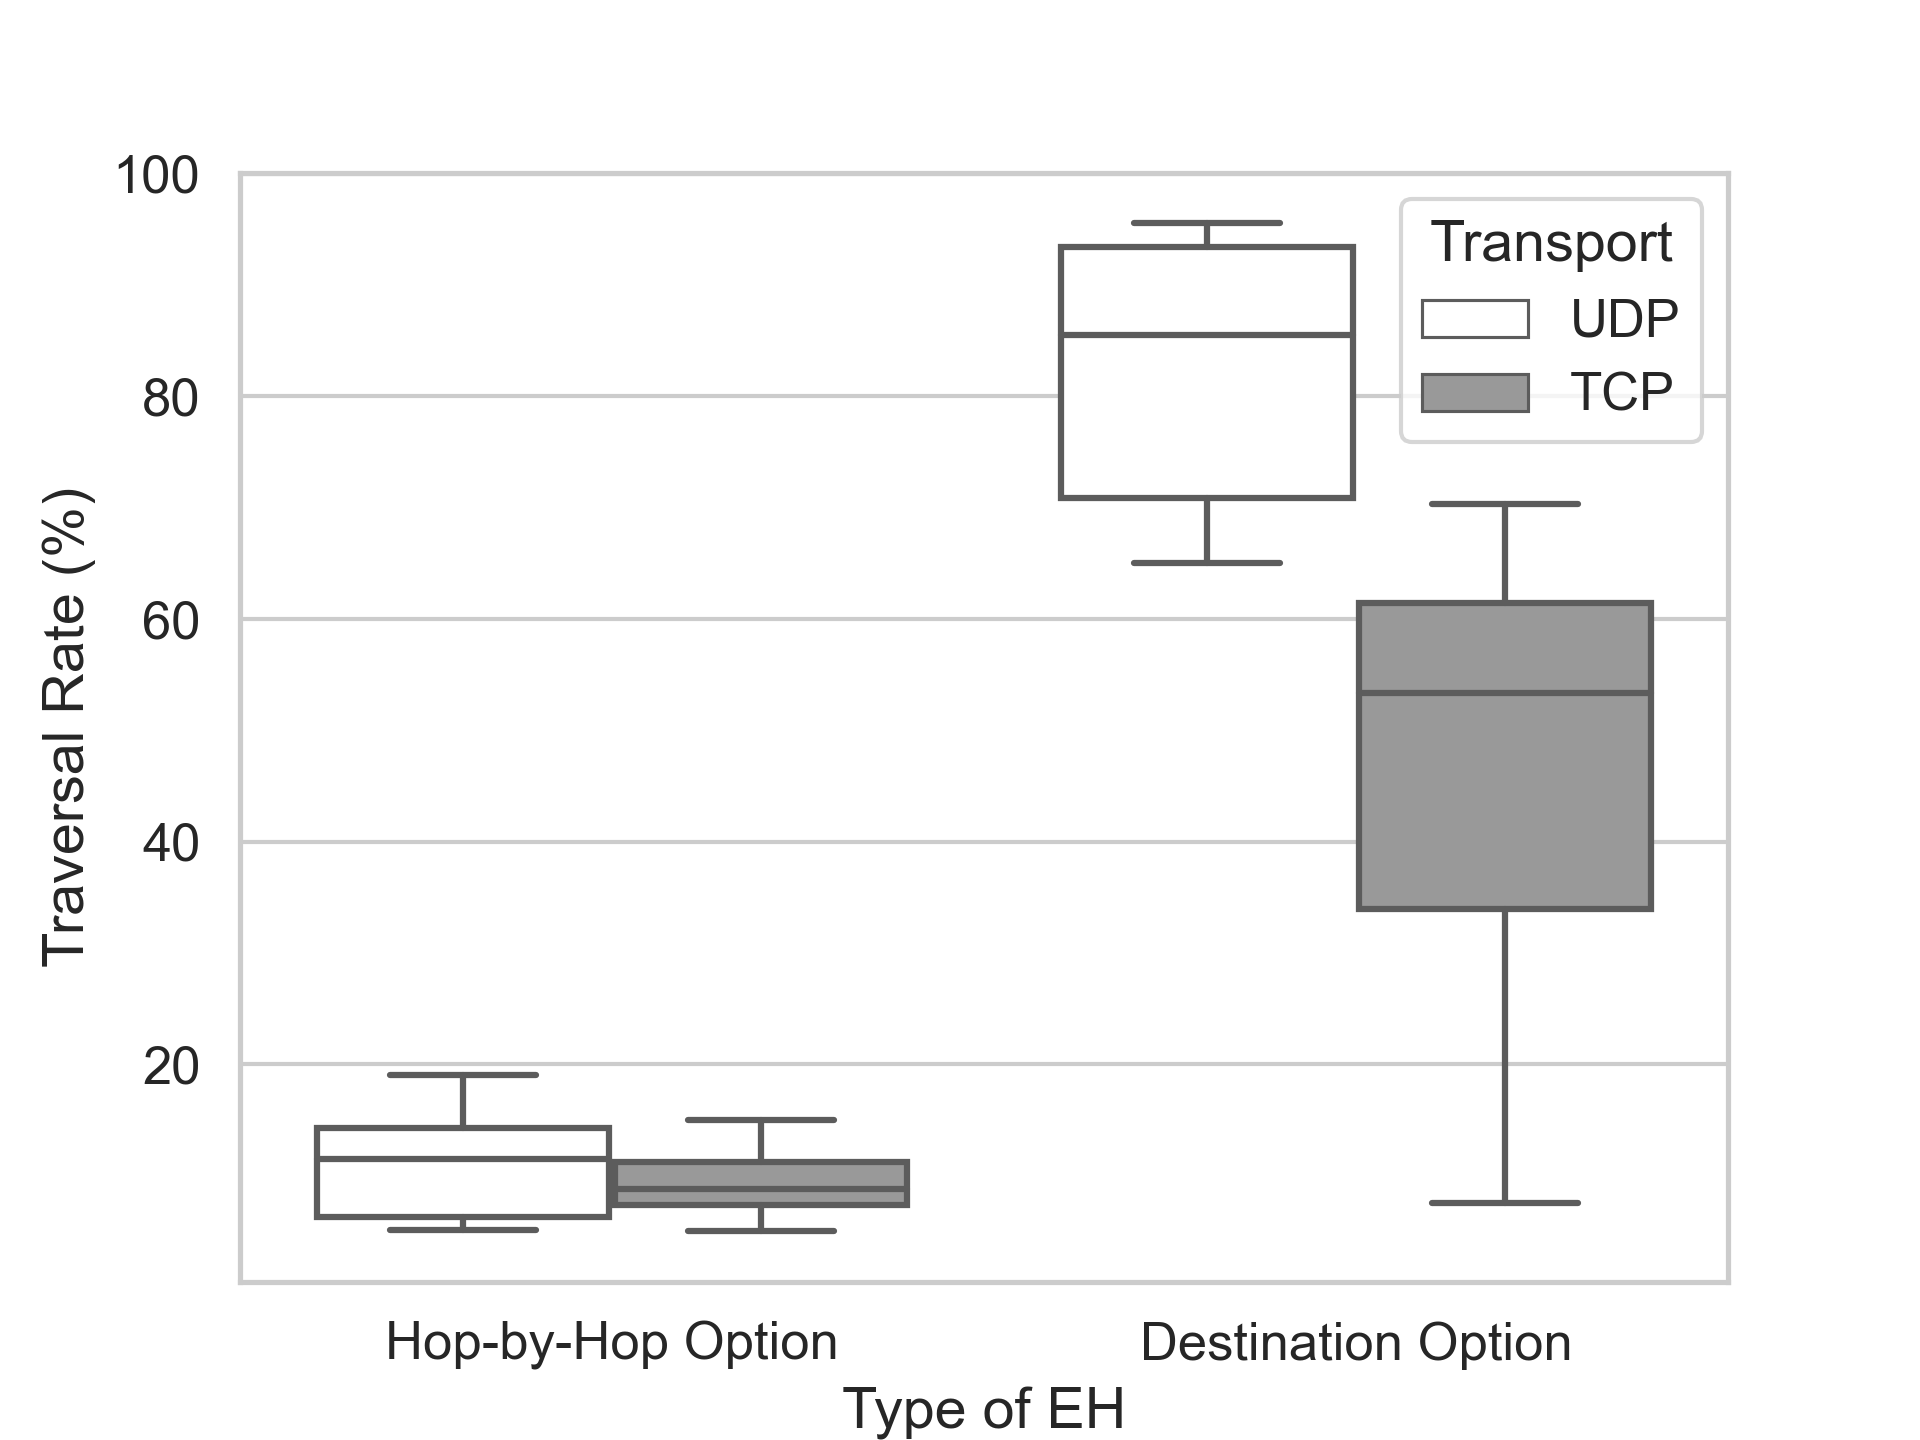
\includegraphics[width=0.5\textwidth]{all_traversal.png}
  \caption{Traversal for packets including HBH and DST, from Atlas vantage points to target servers located in 7 different countries (dataset R1).}
  \label{fig:countrybox}
\end{figure}

In this section, we present the results conducted on the Atlas platform, where
several thousands of vantage points were utilised to target several destinations
in Internet. The primary performance metric analysed is the "traversal rate",
which represents the proportion of paths in which probe packets with EHs
successfully reached the destination AS out of the total paths tested.
Additionally, this section discusses the pathologies associated with the most
critical destinations.

\subsection{Traversal rates to destination AS}

%Prior to each test case, a baseline measurement using vanilla packets was
%carried out and unreachable probes were subsequently removed from the result
%set. 

Figure~\ref{fig:countrybox} shows the distribution of the traversal rate with
four transport header compositions (using DST or HBH extension headers, and
using TCP or UDP), while consistently employing the PadN Option in EHs.  Target
destinations were located in seven countries (the United States (US), the
United Kingdom (UK), Australia, Poland, Zambia, Kazakhstan, and Singapore) using
an average of 4750 vantage points per destination located in RIPE Atlas.

The diagram shows that a substantial number of probes traverse the path when
employing DST EHs, with 83\% and 57\% median number of traversed paths
respectively using UDP and TCP.  However, a relatively lower traversal rate is
observed when using HBH EHs, with medians of 12\% and 9\% over UDP and TCP. In
addition, traversal rates with TCP exhibit much greater variability than with
UDP, ranging from 8\% for Zambian destinations to 67\% for destinations in the
UK.

As discussed later in the paper, the underperformance of HBH EHs, along with
the comparatively lower traversal rate when utilizing TCP, is linked to the
behaviour and configuration of routers within access networks, more
specifically the ISP ingress routers.

To undestand the impact of EH size on the traversal rate, we also conducted an
experiment where IPv6 probes with different header lengths were sent from the
vantage points in Atlas to a server located within the UK's academic network
(JANET).  We utilised EH lengths from 16 to 64~B with 8-byte
increments preserving alignment (dataset R2). The experiment was repeated with
HBH and DST EHs, and using both UDP and TCP.


\begin{figure}[t]
\centering
  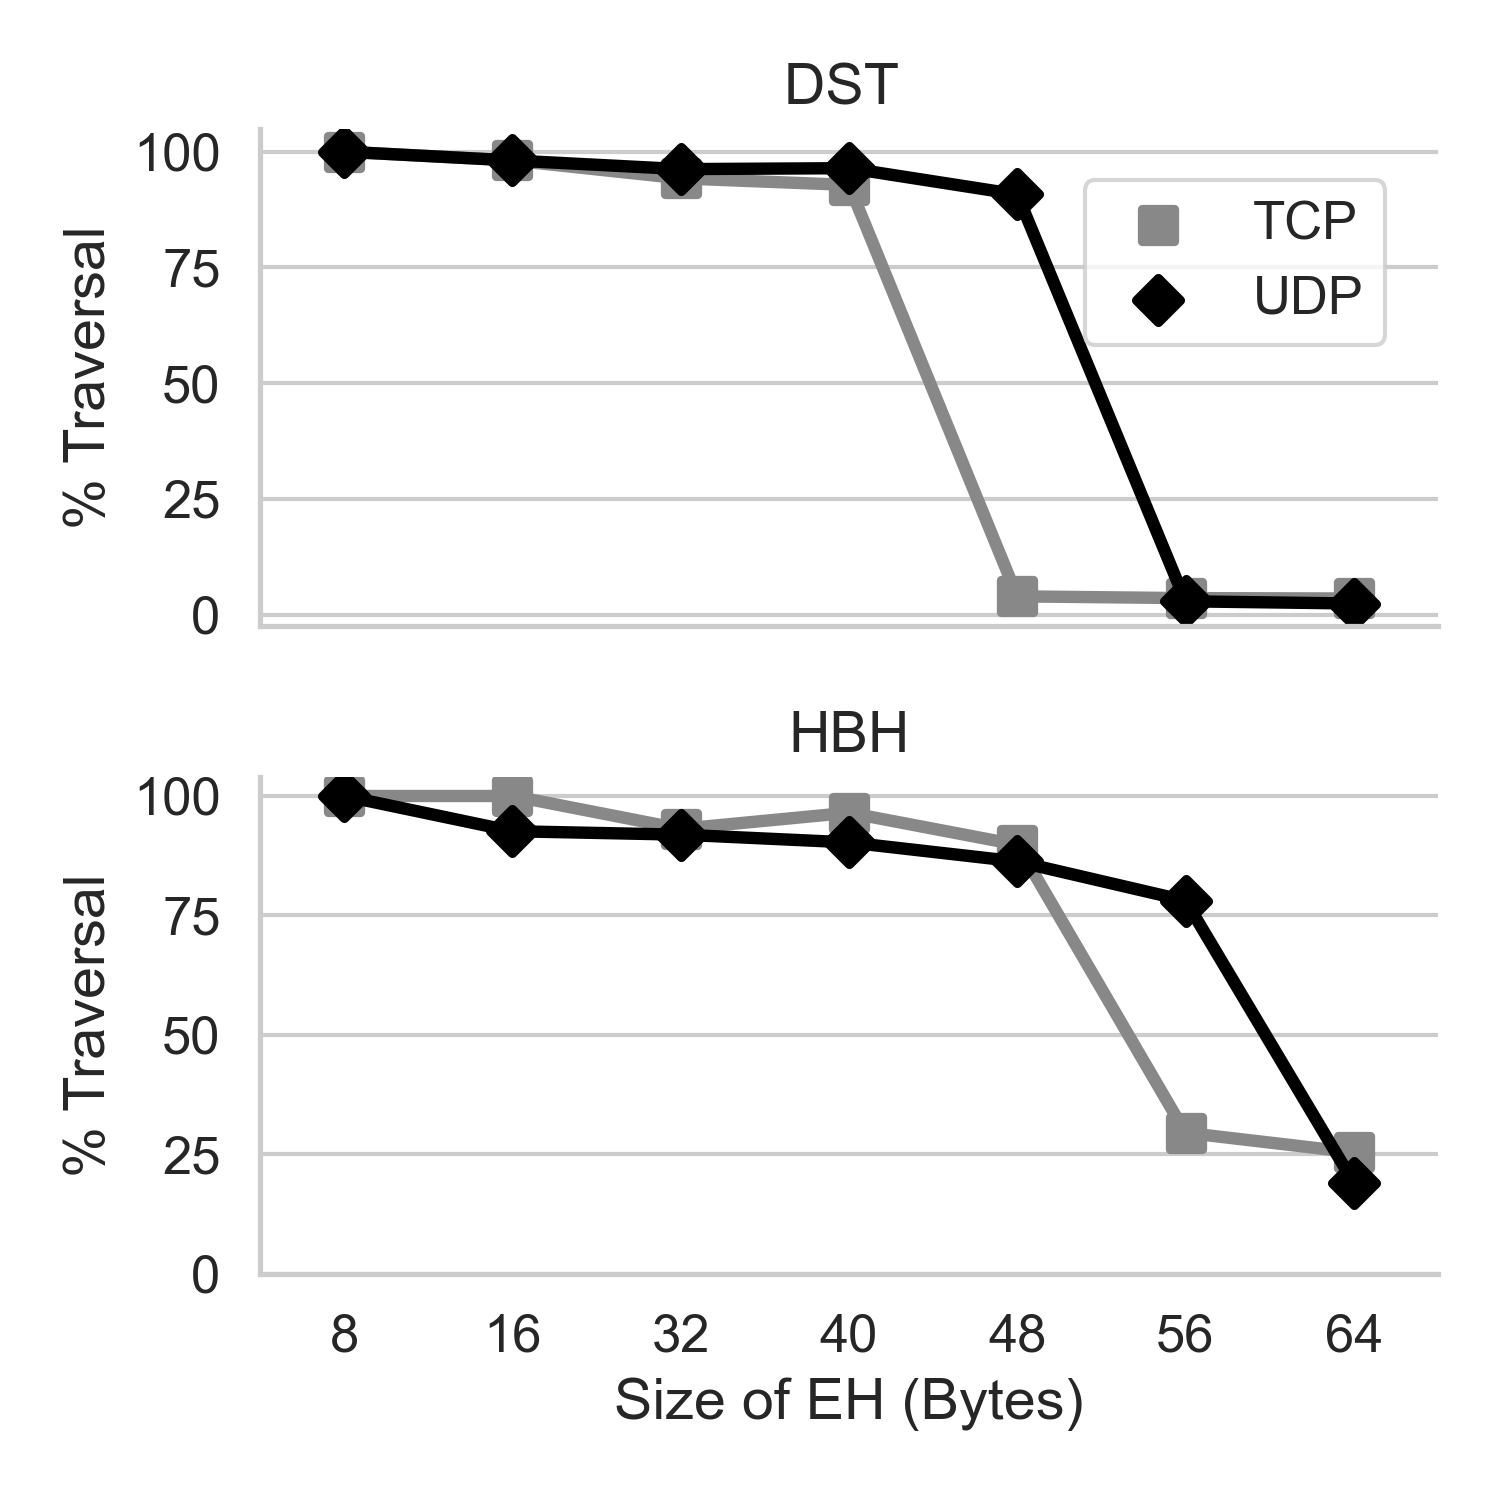
\includegraphics[width=0.45\textwidth]{sizes.png}
  \caption{Traversal rate for packets including HBH and DST EHs from Atlas
vantage points to a target server within the UK JANET network (AS876), shown by
size of EH and split by transport.  Total n=129,585 measurements, with a mean
of 4628 measurements ($\sigma$=351) for each combination of transport, size and
EH (dataset R2). This variation in the number of measurements results from
availability and connectivity of  probes with time.  }

  \label{fig:sizes}
\end{figure}
 

The results depicted in Fig.~\ref{fig:sizes} show the relationship between
header size and traversal rate, demonstrating a decrease in the traversal rate
as the header size increases.  Packets containing a DST EH over UDP exhibit the
most substantial decrease in traversal rate between 48~B and 56~B. A reduction
in traversal rate (2\%) is also observed around the same size for HBH EH. A
comparable pattern is observed in TCP experiments, where the most significant
drop occurs between 40~B and 48~B, representing a header size 8~B smaller than
UDP.

We can relate the difference in traversal rate between UDP and TCP to the overall
size of the transport header.  The combined header size of TCP (20~B) and IPv6
(40~B) with a 48~B EH is 108~B, while the combined header size of UDP and IP
with a 56~B EH is 104~B. This suggests that, for this particular test, 104~B
serves as an upper limit of the transport header beyond which paths are more
likely to experience a significant increase in packet drops. These findings
align with the results reported in~\cite{james-imc}, which examined traversal
rates for DST EHs of sizes 32B and 64B, and identified traversal drops
specifically at the 64~B EH size.

As indicated in~\cite{james-imce}, the sharp decline in traversal rates for
headers larger than 104~B is primarily caused by the router's limited buffer
for header processing, leading to the dropping of oversized headers.
These buffers could potentially impose constraints on the future usability of
large IPv6 extension headers.


%%% this size is strctly less than the size of the end-host parsing bufer
%[ref?]

\begin{figure}
\centering
  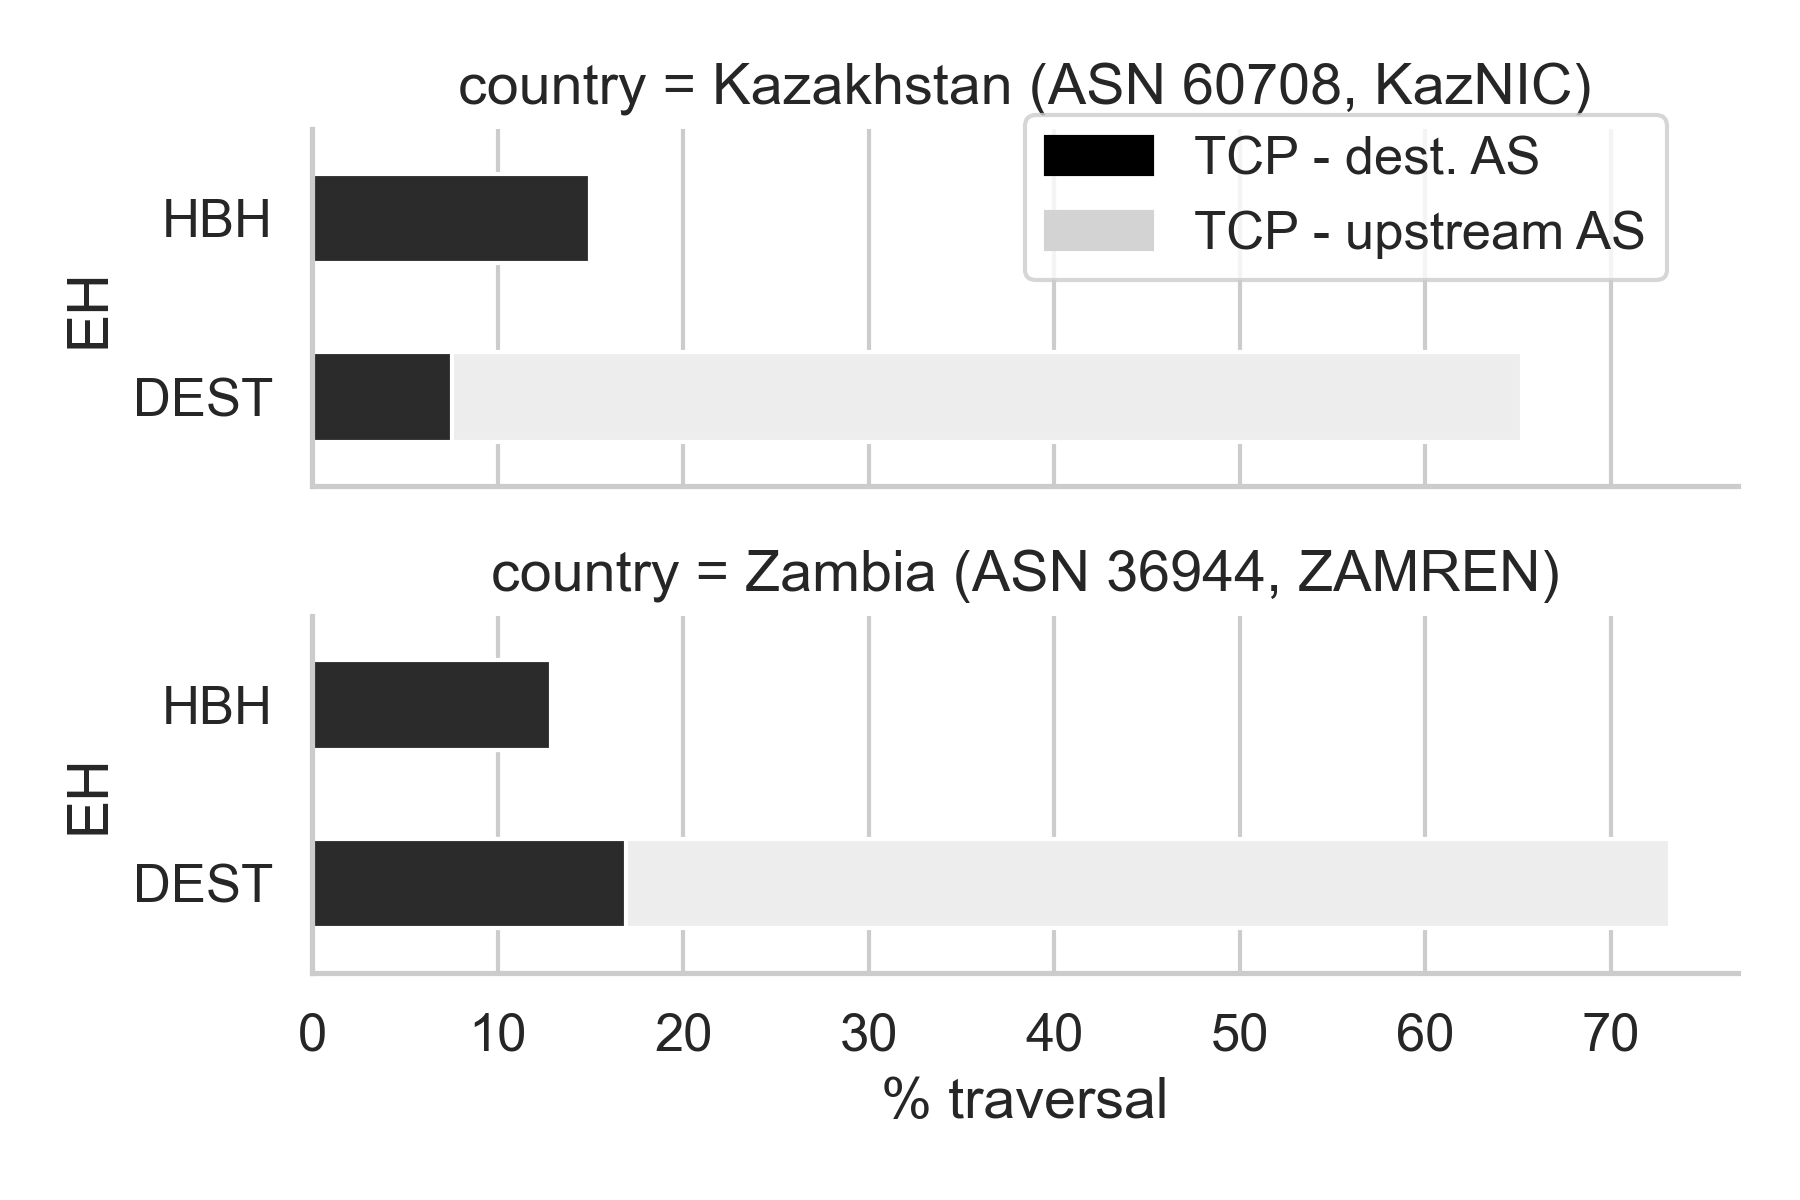
\includegraphics[width=0.5\textwidth]{traversal-pathologies.png}
  \caption{Traversal from Atlas vantage points to both destination and upstream
AS for targets in Kazakhstan (n=5075) and Zambia (n=4462). The figure shows the
traversal percentage of TCP packets using both types of tested EH.}
  \label{fig:traversal_pathologies}
\end{figure}

\subsection{Effects of Tunneling}
    \label{subsec: pathologies}

In some pathological cases, the traversal rate of HBH EHs can be significantly
affected by strict traffic aggregation policies enforced network operators.

Two notable examples in our traces are the Kazakhstan and Zambian network.
Both destinations are reachable from Atlas only through a single BGP peer
(Border Gateway Protocol) and see the majority of packets dropped at the
second to last AS on their path (corresponding to the destination's upstream AS).
While the traversal rate to the destination's upstream AS shows behaviour
similar to other destinations (see Fig.~\ref{fig:traversal_pathologies}),
the traversal rate to the target AS is significantly diminished. This indicates a
severe blockage at the tunnel entry point.

% where Hurricane
% Electric (AS6939) serves as the sole BGP (Border Gateway Protocol) peer. This
% network employs a brokering service that tunnels IPv6 peering over an existing
% IPv4 connection to an endpoint situated in Dusseldorf.

Upon closer examination, we found that nearly all the paths from the
Khazakhstan network that allow DST EHs to go through originate from ASes
located in Australia or New Zealand. Conversely, packets originating from other
geographical areas are filtered at the tunnel endpoint. This is a specific
pathology due to a potential misconfiguration or policy within the operator's
transit network.

%They can also come from comcast but somehow they bypass HE?!?!?!?!

Similarly, the only BGP peer connecting the target AS in Zambia is Ubuntunet
Alliance for Research and Education Networking.  Notably, there is no shared
origin for the paths where packets successfully traverse from this AS,
indicating that the drops associated with this destination are likely
attributed to an operator policy.

\begin{table}
\centering
%\caption{Per-AS drop attribution for 8~B DST packets sent from n=4970 Atlas vantage points to a target destination in AS786. The local AS is responsible for the majority (5\% for UDP and 25\% for TCP) of the drops.}
\caption{Traversal rates at ASes along the path}

\begin{tabular}{l|c|c|c|c|c}
   AS     & $1^{st}$  & $1^{st}\rightarrow 2^{nd}$   & $2^{nd}$  & $2^{nd} \rightarrow 3^{rd}$ &   $\infty$ \\ 
\hline \hline
DST UDP  & 95.3\%   & 93\%     &          &          & 91.5\%  \\
DST TCP  & 74.7\%   & 70\%     &          &          & 68.5\%  \\\hline
HBH UDP   & 31.4\%   & 20.1\%   & 15\%     & 12.2\%   & 11.4\%  \\ 
HBH TCP   & 26.9\%   & 16.3\%   & 13.9\%   & 9.7\%    & 8.6\%   \\ 
\end{tabular}
\label{tbl:uk_as1}
%\bigskip

%\caption{Per-AS drop attribution for 8~B HBH packets sent from n=4970 Atlas
%vantage points to a target destination in AS786. The local AS is responsible
%for the majority (68\% for UDP and 74\% for TCP) of the drops.}
%
%\begin{tabular}{p{0.07\textwidth}|l|l|l|l|l}
%
%              & 1st AS & AS1\textgreater{}AS2 & 2nd AS & AS2\textgreater{}AS3 & $inf$     \\ \hline
%HBH UDP & 31.4\% & 20.1\%               & 15\%   & 12.2\%               & 11.4\% \\ \hline
%HBH TCP & 26.9\% & 16.3\%               & 13.9\% & 9.7\%                & 8.6\%  \\ 
%\end{tabular}
% \label{tbl:uk_as2}
\end{table}


\subsection{Analysis of drops along the path}

We now shift our focus to identifying the specific points along the path where
drops of packets carrying EHs are most likely to occur.

Table~\ref{tbl:uk_as1} presents the traversal rate at different stages of the
path, starting from the vantage points in Atlas and leading to the UK target.
Within this table, the columns labelled as $1^{st}$, $2^{nd}$, and $\infty$
represent the traversal rates measured within the first, second, and last AS.
Additionally, the columns labelled $1^{st}\rightarrow 2^{nd}$ and
$2^{nd}\rightarrow 3^{rd}$ indicate the traversal rate at the peering point
between ASes.

As expected, as probes traverse the network the traversal rate
progressively decreases.  However, the majority of HBH EHs (68\% UDP, 74\% TCP)
and a noteble fraction of DST EHs (5\% UDP, 25\% TCP) are dropped within the
initial AS, i.e.  within the AS where the vantage point is located.  This
pattern of loss is observed also when data is analysed per AS.

Packet drops within the initial AS are prevalent to all Atlas measurements,
irrespective of the destination. However, packets carrying DST EHs over UDP
experience a drop rate less than 1\%, as they travel across further ASes.  This
suggests that, once the Internet core is reached, EHs can travel to the
destination with minimal disruption.

\begin{figure}[t]
\centering
  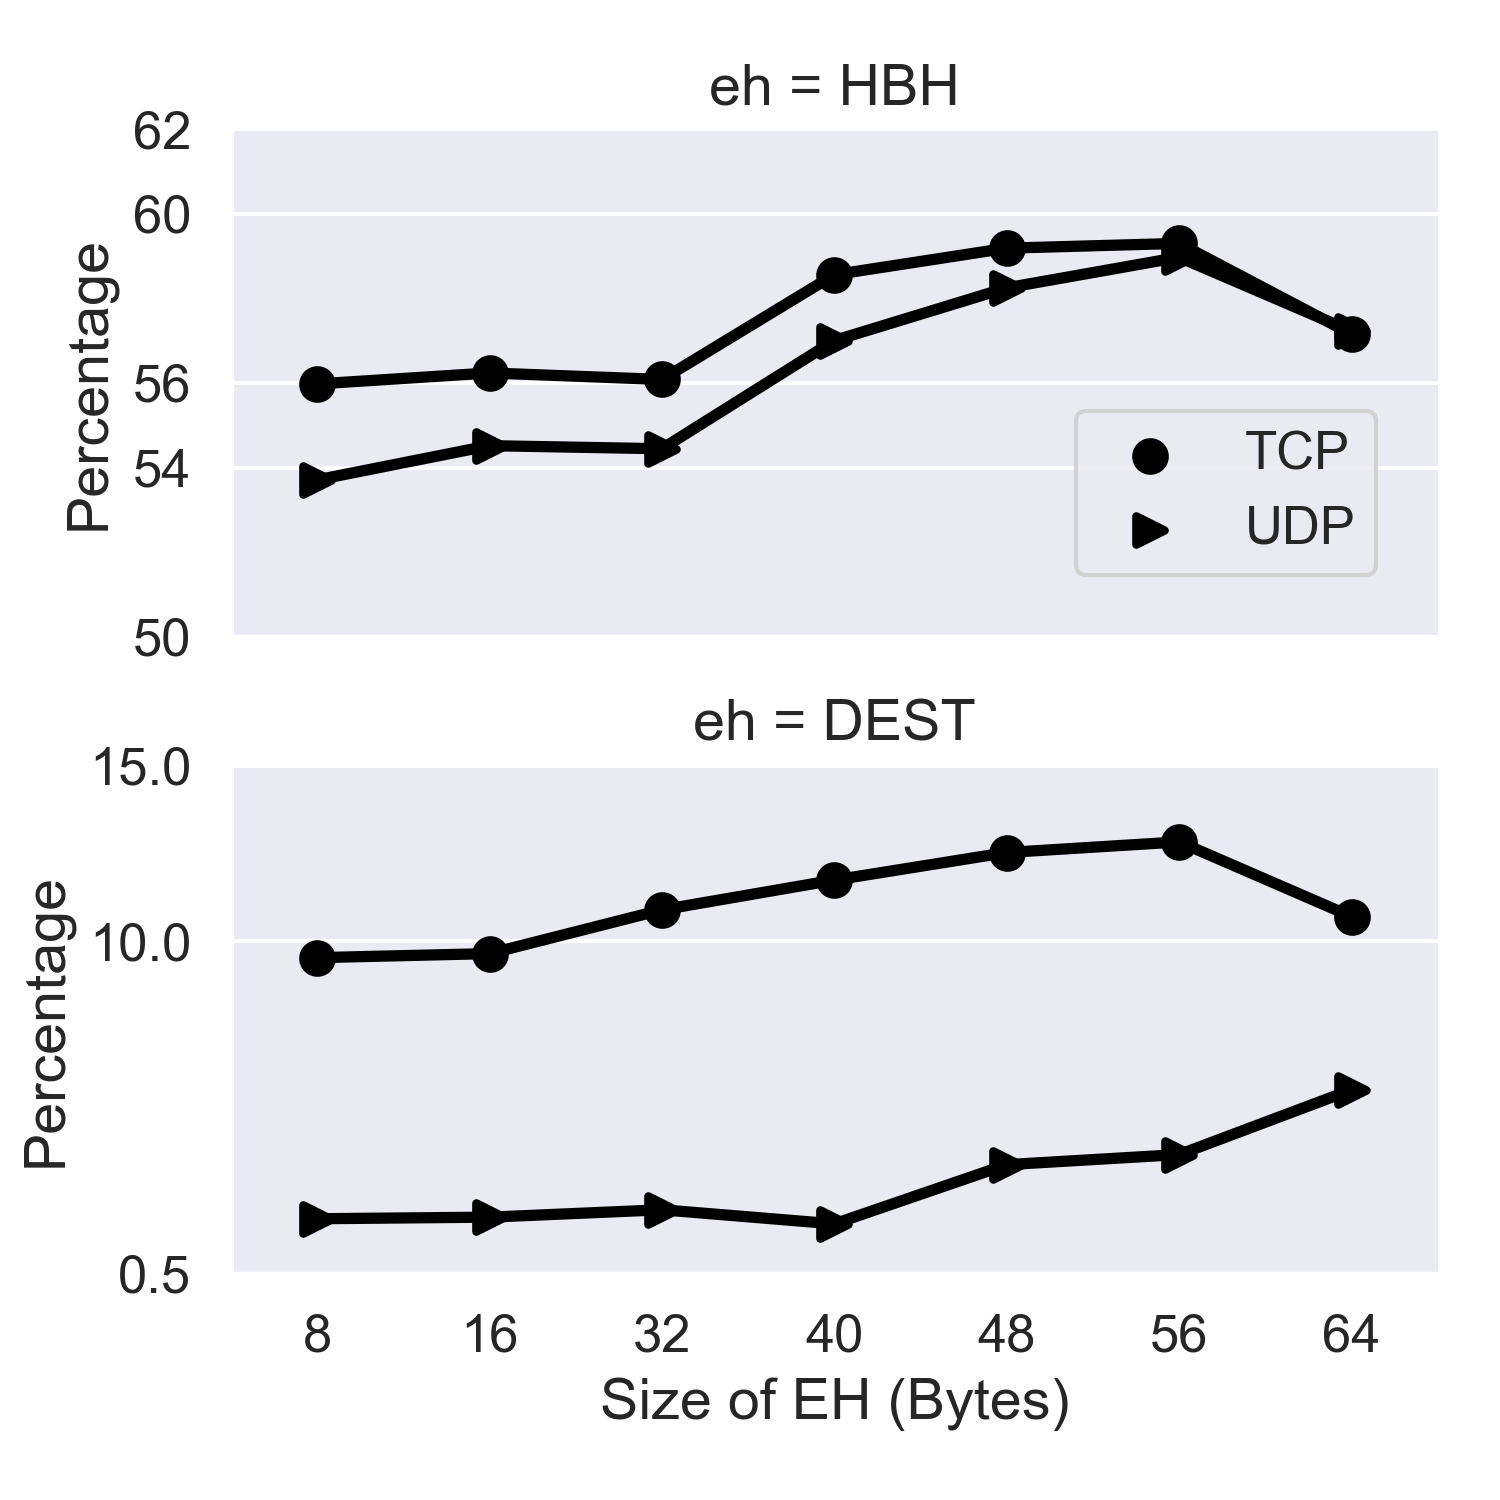
\includegraphics[width=0.5\textwidth]{empty_paths.png}
  \caption{Percentage of paths with drops at the first router.}
  \label{fig:empty_paths}
\end{figure}

\subsection{EH drops at local router}

Upon further investigation, we found that the majority of drops in the first AS
in fact occurs at the very first router on the path, specifically the vantage
point's local upstream router.

To appreciate how prevalent are packet dropped at the first router with respect
to the overall drops, Figure~\ref{fig:empty_paths} shows the percentages of
paths where packets are discarded at the first router as a function of the
header size.  These are paths where no traceroute responses are received for
test packets with EHs, but responses are received for control packets without
EHs.

Packets containing a HBH EH are dropped at the local router for over 50\% of
the paths, whereas a significantly lower drop rate is observed for packets with
DST EHs.  Also, we observe that the type of transport has minimal influence on
the outcome for HBH EHs (54\% UDP, 56\% TCP), but is more important for DST EHs
(2.5\% UDP, 10\% TCP).

It is noteworthy that the loss rates associated with header size at the first
router do not display a sudden shift at a specific EH length, as previously
illustrated in Figure \ref{fig:sizes} for the overall path. Instead, they
exhibit a more consistent pattern across the entire range of EH lenghts under
examination.  This behavior can be attributed to the distinct architecture of
access routers, which differs significantly from that of core routers and
imposes fewer constraints on the buffer allocated for header processing.

% The percentage increases with size  is regardless
% of which EH was included.

Edge routers deployed at vantage points commonly serve the purpose of
connecting enterprise LANs, mobile networks, and broadband networks. These
routers fulfill multiple functions, including access control and
authentication, which often require access to the complete transport header.
Consequently, they tend to prioritise flexibility in handling transport headers
over speed.

In order to understand the impact of access routers, we examined the
relationship between EH dropping and MSS (Maximum Segment Size) clamping, a
common technique employed by edge routers to circumvent the need for path MTU
(Maximum Transfer Unit) discovery~\cite{custura-mtu}.  MSS clamping involves
the intermediate router to insert a TCP Option into the TCP handshake segments
to ``clamp" the MSS utilised during the connection to a suitable value for the
network.

Given that endpoints in Atlas do not use the MSS Options by default, the
presence of an MSS Option at the destination indicates that an intermediate
router inserted it. This implies that the intermediate router likely analysed
the complete TCP/IP header to identify the insertion point and fabricated a new
header, potentially resulting in the dropping of packets with unknown EHs.

% We do not have a way to determine whether a drop is a result of a configured
% policy, a bug, or a lack of support.  However, it is possible to identify paths
% that insert/modify a TCP option by using a traffic capture tool to examine the
% measurement packets as they arrive at the destination server during the
% baseline measurement. 

% By default, the packets sent from an Atlas probe does not
% include a TCP MSS option - when Option is present at the destination, this
% means a node on that path has inserted this. 

In our traces, we identified 853 paths where an on-path router inserted a TCP
MSS option during our baseline measurements towards the UK destination. Within
this subset of paths, the traversal rate for HBH EHs is merely 2.6\%, while for
DST EHs, it stands at 48.1\%. The chi-square test (p-value$<10^{-43}$) gives
strong evidence of a correlation between EH drops and MSS clamping, indicating
that drops occur more frequently when, to modify the TCP MSS Option, an on-path
router must traverse the chain of EHs. 

%% NB: p-values have been calculated using "scipy" in Python

% observed_DST = [[442, 1124], [411, 2993]]
% observed_HBH = [[883, 728], [15, 3389]]
% chi2, p_value_DST, _ , _ = scipy.stats.chi2_contingency(observed_DST)
% chi2, p_value_HBH, _ , _ = scipy.stats.chi2_contingency(observed_HBH)

% We then look at EH traversal within this subset of paths, to determine whether
% this results in a difference to the overall traversal, on the basis that at
% least one on-path router will have needed to parse the entire IPv6 Header,
% including any EHs, to perform this function.  

\subsection{EHs and router forwarding behaviour}

In our tests, we aimed at investigating whether the use of EHs results in a
discernible change in forwarding behaviour compared to scenarios without EHs.
It is well known that load-balancing routers can be configured to use
layer-3 and layer-4 headers for routing purposes. Additionally, many ECMP
(Equal Cost Multi Path) routers distribute traffic on different paths based on
a digest that includes the Next Header field (NH) in
IPv6~\cite{lb-classification}.  Misinterpreting NH can result in forwarding
packets of the same flow, both with and without EHs, along different paths,
leading to detrimental reordering effects.

% The objective of these test was to assess whether routers, which base their
% forwarding decisions on the packet structure, exhibit altered behavior when
% handling packets containing EHs. Our findings substantiate this case,
% highlighting the potential impact of end-to-end use of EHs on network
% utilization.
% 

% Some routers can be configured to select a path based on the Flow Label field
% in the IPv6 header In this case, adding an EH to a packet within a flow would
% not result in reordering.

Paris Traceroute was used to determine if the choice of a path is affected by
the presence of an EH.  This tool detects the presence of a load balancer on a
given path by performing several traceroute measurements between the same
source-destination pair and varying a predetermined set of fields called a
\textit{Paris variation}~\cite{augustin2006avoiding}.  Packets belonging to the
same Paris variation are identified by either a range of sequence numbers in
TCP or the checksum in UDP.

% A router could be designed to use
% various sets of fields for load-balancing~\cite{lb-classification}.

Paris Traceroute measurements were conducted from the vantage points under our
control in Atlas to the destination in Zambia.  A vantage point was included in
this analysis only if consistently successful in previous tests.  In total, 766
paths were included.  Each run between a source and a destination pair was repeated 6
times and comprised 16 Paris variations, each with a different configuration of
the IPv6 Flow Label and transport port number.  These same 16 configurations
were used in all the measurements. 

%Six sets of measurements were run from all vantage points to the Zambian
%destination, with each set of measurement using 16 Paris variations. We select
%the vantage points and destination based on previous measurements, so as to
%only measure complete paths, where traversal always succeeds, 766 paths in
%total.

% The version of Paris Traceroute that was used allowed to deterministically set
% the IPv6 Flow Label and transport port number for measurement in a group of set
% of 16 Paris measurements. The same 16 combinations of IPv6 Flow Label and port
% number were used for subsequent measurement sets.

\begin{figure}[t]
\centering
  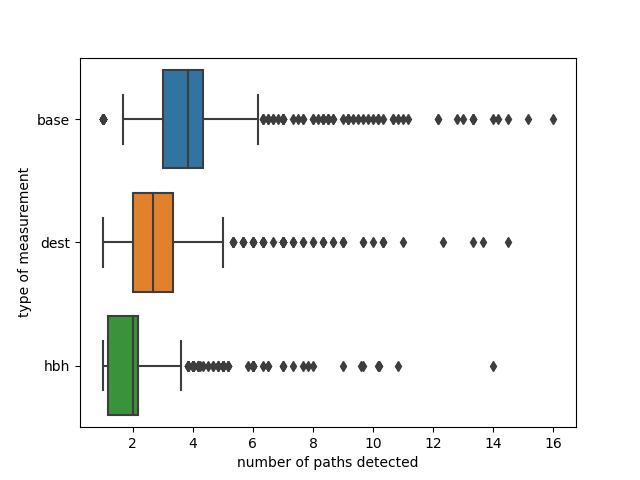
\includegraphics[width=0.5\textwidth]{boxplot-paths-detected.png}
  \caption{Number of paths detected by Paris Traceroute in 866
source-destination pairs, averaged over 5 measurement runs, with each run using
the same 16 Paris variations. The baseline measurement using packets with no EH
is compared against packets including DST and HBH measurements (dataset R3).}
  \label{fig:paths-detected}
\end{figure}

Figure~\ref{fig:paths-detected} compares the distribution of the number of
alternative paths discovered by Paris Traceroute including all
source-destination pairs and Paris variations.  The baseline distribution is
compared to the one obtained when a DST EH or a HBH EH was inserted into the
IPv6 header.  A median of 4.1 paths in the baseline experiment matches the
results in~\cite{augustin2006avoiding}.  However, when DST EHs and HBH EHs are
inserted, the medians reduces to 2.96 and 2.1 paths respectively.  


% p-value is calcuated assuming null hypothesis

The variation in the number of identified paths suggests that the inclusion of
an EH influences significantly the forwarding behaviour of routers along the
tested paths.  When analysing individual source-destination pairs, the
measurerement with a DST EH detected the same number of paths as the baseline
(within 1 path) in 60\% of cases and fewer paths (by less than 1) in 38\% of
the cases.  The measurement with HBH EHs was even more compelling with 13.4\%
of source-destination pairs with the same number of alternative paths and
69.7\% having less paths than the baseline.

These results highlight that when EH shifts the position of the headers
following the baseline IPv6 header, the router is compelled to make different
routing decisions.  For example, if the hash calculations for path selection
rely on extracting the transport port from a fixed offset, instead of correctly
parsing the IPv6 header chain, the inclusion of an EH may result in reduced
entropy of the data.  This, in general, limits the options of ECMP-enabled
routers and potentially leads to congestion and path overloading.

%%%%%%%%%%%%%%%%%%%%%5

% For some source-destination pairs, the EH Paris measurements detect at least 1
% more path than for a packet with no EH. 

Although less common (around 1\% of the cases), for specific paths, the introduction
of an EH resulted in a significant increase in the number of alternative paths,
far surpassing the count observed without EH.
For example, in one case, the baseline measurement detected 4 paths, the DST
measurement found 2 paths, and the HBH measurement uncovered 14 paths. This
unusual behavior was observed due to a single router exhibiting 14 interfaces
when handling packets with HBH EHs. While it does not significantly impact
overall usage, it deviates from expected behavior.

Finally, for some source-destination pairs in our dataset, we observed packet drops
specifically for paths that included an HBH EH, indicating inconsistent
traversal for packets with this EH. These measurements also reveal that HBH and DST
EH packets are forwarded in the same way as packets without EHs on only 13\%
(for HBH) and 60\% (for DST) of paths, highlighting the potential impact of EHs
on load-balancing router functionality.


%For 12 source-destination pairs in the dataset, not enough data was gathered
%using Destination Option EHs to complete a measurement run. Not enough data
%was gathered for 137 (15.8\%) pairs.

 
\section{PATHspider results} 
\label{sec:pathspider-results}
%~\cite{learmonth2016pathspider} 

This section presents results from the analysis of the PATHspider dataset.
These experiments measure the end-to-end traversal rates of EHs from a small
pool of vantage points (5 worldwide locations) to a large number of web and
DNS servers.  Unlike the results based on the Atlas dataset, in these
experiments we require the server to process the packet containing the EH and
reply to it. Thus, the traversal rate in these tests also accounts for the ability
of the destination to process an EH.

The IPv6 addresses of the target web servers in these tests were collected by
resolving the domain names in the Cisco Umbrella top 1M list. The IPv6
addresses of the DNS servers, instead, were obtained considering the list of
authoritative name servers for the same list of domains.

A run of the experiment consisted in sending an IPv6 probe packet, either a DNS
query over UDP to a DNS server or a TCP SYN to a web server, and observing the
corresponding reply.  The test was marked as successul if a reply was received
both with and without EHs, which indicates that the path existed and could
support a certain type of EHs.  The tested EHs were DST and HBH with a PadN Option.

%This section reports the end-to-end support percentage, indicating the paths
%where test packets receive a response from the destination server.

\begin{table} 
\centering
\caption{Server support for DST and HBH EHs (Feb 2023). }
\begin{tabular}{p{1.5cm}|cc|cc}
\multicolumn{1}{l|}{} & \multicolumn{2}{p{2cm}|}{\centering DST support} 
                      & \multicolumn{2}{p{2cm}}{\centering HBH support} \\ \cline{2-5} 
\multicolumn{1}{l|}{} & \multicolumn{1}{c|}{TCP}   & UDP      & \multicolumn{1}{c|}{TCP}     & UDP   \\ \hline \hline
UK                    & \multicolumn{1}{c|}{69.1}  & 69.3     & \multicolumn{1}{c|}{12.5}    & 15.8  \\ \hline
Canada                & \multicolumn{1}{c|}{76.3}  & 76       & \multicolumn{1}{c|}{23.3}    & 24.2  \\ \hline
Australia             & \multicolumn{1}{c|}{72.5}  & 72.2     & \multicolumn{1}{c|}{17.7}    & 17.5  \\ \hline
Singapore             & \multicolumn{1}{c|}{72.8}  & 72.7     & \multicolumn{1}{c|}{17.4}    & 17.4  \\ \hline
Poland                & \multicolumn{1}{c|}{76.5}  & 76.8     & \multicolumn{1}{c|}{24.4}    & 24.7   
\end{tabular}
\label{tbl:e2e_traversal}
\end{table}


\begin{table} 
\centering
\caption{Support for DST and HBH EH from DNS providers (Dec 2022).}
\begin{tabular}{l|c|c|c}
           & \% of dataset &  DST support & HBH support\\
\hline \hline
Cloudflare & 18   & Yes  & No                 \\
\hline
Amazon     & 11   & No   & No                 \\
\hline
Hetzner    & 3    & Yes  & No                 \\
\hline
Gandi      & 4    & No   & No                 \\
\hline
Ionos      & 3    & Yes  & No                
\end{tabular}
\label{tbl:provider_support}
%Google does not support either EH, and is not listed in the table because it was only 30 destinations in the dataset.
\end{table}


\begin{table} 
\centering
\caption{Support for DST and HBH from web providers (Dec 2022).}
\begin{tabular}{l|c|c|c}
           & \% of dataset & DST support & HBH support\\
\hline
\hline
Amazon       & 52                     & Yes                & No                 \\
\hline
Cloudflare   & 23                     & Yes                & No                 \\
\hline
Akamai       & 2.7                    & Yes                & No                 \\
\hline
Google       & 2.3                    & No                 & No                 
\end{tabular}
\label{tbl:web_providers}
\end{table}


\subsection{End-to-end support}
\label{subsec:e2esupport}

Table~\ref{tbl:e2e_traversal} shows the percentages of successful tests with
the DST and HBH EHs to DNS servers (UDP) and web servers (TCP).  Inline with
previously presented data, support for DST EH is higher than HBH EH, with
69-77\% of the tested servers replying when including DST compared to only
12-25\% when including HBH.  However, unlike the results from Atlas database,
these statitics are only marginally affected by the type of transport protocol
(UDP or TCP).  The similarity between UDP and TCP can be attributed to the
absence of specific router configurations, such as CPEs, along the path that
are instead more prevalent in access networks.

% We find more than two-thirds of Amazon-hosted webservers respond to connections
% by packets including DST, whereas Amazon-hosted DNS servers has no EH support. 

Interestingly, the table also reveals more significant variations of HBH EH
success rates than DST EHs when servers were probed from different vantage
points. For instance, the support for HBH EHs varies from 12\% from a UK
location to almost 25\% from a Polish site.  This indicates that the transit
network may have a greater impact on blocking HBH EHs than DST EHs.  

% Overall end-to-end EH
% support for web servers in the dataset range from 72 and 78\% for DST EH and 2
% to 3\% for HBH EH.

%Only one measurement, from the Singapore vantage point, observed a 5\%
%difference based on transport in favour of TCP for both tested EHs. 

It should be noted that the  majority of web servers and at least one-third of
DNS servers in our traces were managed by a few major hosting companies, such
as Cloudflare\texttrademark and Amazon\texttrademark.  Tables
\ref{tbl:web_providers} and \ref{tbl:provider_support} provide a ranking of the
hosting companies based on the share of hosted IP addresses for web and DNS
servers, respectively. The tables also report the policy adopted by these
companies regarding the propagation of packets including DST and HBH EHs.  

As we can see, large companies tend to enforce stringent filtering policies to
packets that include EHs, possibly because they feel more exposed to potential
risks of incorrect handling of EHs.  We found that the policies implemented by
the larger hosting providers have indeed the greatest impact on the global
traversal rate of packets with EH. 

%Our analysis conducted in Feb 2023 found a total of 232,350 IP addresses, the
%majority of which are provided by a few hosting companies: around 52\% of
%destinations were hosted by Amazon Inc, 23\% by Cloudflare, and 2.5\% were
%hosted by Akamai Technologies and Google.  Table~summarises the  EHs for each
%hosting company.

% In order to consider the influence of the major hosting providers,
% Table~\ref{tbl:provider_support} presents the DST and HBH EH support for the
% largest DNS providers in our dataset, along with their incidence.  

To appreciate this impact, consider that in early December 2022, a change of
policy in Cloudflare\texttrademark allowed servers to respond to DNS queries
carrying EHs.  As a result, there was a dataset-wide increase in success rate
from 57\% to 70\%, as currently reported in the table.  Extrapolating from
this, if all the major providers were to enable support, we estimate that the
success rate of this test would exceed 90\% for DST and 60\% for HBH.


\subsection{Analysis of AS support for EHs}

\begin{table}
\caption{AS reachable by DST or HBH EHs (Dec 2022).}
\begin{tabular}{l|c|c}
Supported EH                & Paths per AS$>$=1 & Paths per AS$>$=10 \\
\hline \hline
Total  ASes                 & 2787              & 1606 \\
\hline
%No DST support             & 212 (7.6\%)        & 110 (6.8\%)    \\
DST on at least 1 path      & 2575 (92.4\%)     & 1496 (93.2\%)      \\
DST on at least 50\% paths  & 2476 (88.8\%)     & 1437 (89.4\%)      \\ \hline
%AS does not support HBH  & 1287 (46.2\%)  & 709 (44.1\%)            \\
HBH on at least 1 path      & 1500 (53.8\%)      & 897 (55.9\%)      \\
HBH on ar least 50\% paths  & 1037 (37.2\%)      & 580 (36.1\%)  
\end{tabular}
\label{tbl:as_pathspider}
\end{table}

If we consider the traversal rates of EHs in ASes, the outlook is different.
Table~\ref{tbl:as_pathspider} reports the  number of ASes containing the target
DNS servers that could be reached from at least a vantage point over at least a
path and compares it with the total number of ASes (2nd column) discovered in
the trace. To assess that this same metric is valid across multiple paths to
the AS, we also report the number of AS reachable over a least 10 paths (3rd
column), and those that succeed in more than half of paths in both DST and HBH
cases (3rd and 5th row, respectively).

%Tablepresents the traversal
%rates for the ASes targeted by PATHspider (2868 in total). 

% from at least one of the vantage points.
% a target server belonging to the AS probed f
% The first column considers all destination ASes in the dataset, while the
% second only looks at ASes that host 10 destination addresses or more. 

It is worth noting that these estimates of the actual support of EHs in ASes
are conservative, as the destination ASes that were not reachable from any
vantage point may have been masked by upstream ASes dropping EHs.

% alongside evidence that they support either the DST or HBH EH.  If at
% least one reply is seen from an AS to one of our test packets from any of the
% locations tested, we consider that AS supports the traversal of packets that
% include the tested EH type. 

These figures clearly highlight that transparent delivery of EHs is common
among the majority of ASes: overall, about 90\% of ASes allow
traversal of packets including an 8~B DST EH, and about half of ASes allow an
8~B HBH EH.  When considering the ASes (1606) tested over 10 or more paths, the
results vary little.  This suggest that DNS servers are more concentrated in
ASes with stricter policies.

The presented figures reduce when packets travel towards the destination
through multiple ASes, suggesting that many packets that include an EH could be
dropped well before reaching the destination AS. For DST, 3.4\% fewer ASes
permit DST traversal on more than half the paths, whereas for HBH, the
difference is 16.6\%. Again, this demonstrates the importance of the transit 
network in supporting HBH EHs. 

\subsection{Support for EH Options}

\begin{table}[t]
\centering 
\caption{Support for EH Options in DNS queries.}
\begin{tabular}{l|c|c}
Test                      & DST support & HBH support\\
\hline \hline
Pad N Option (1)          & 69.3        & 15.1       \\
PMTU Discovery (48)       & 69.5        & 15.8       \\
Experimental Option (30)  & 69.4        & 15.1       \\
Experimental Option (254) & 0.4         & 0          \\
Incorrect Option Length   & 0.5         & 0.05            
\end{tabular}
\label{tbl:option_type_support}
\end{table}

Additional measurements were conducted to determine whether the findings
presented can be observed across other Options within EHs.  In particular, we
evaluated the effect of the two higher ordered bits of the Option type
that indicate how router should behave when the option is unknown.

Table~\ref{tbl:option_type_support} shows the percentage of support for various
Option types in tests towards DNS servers.  In addition to the already
considered PadN Option, we tested the recently standardised MinPath MTU
HBH~\cite{rfc9268}, and two experimental Options, namely 30 and
254~\cite{RFC4727}.  The latter has been defined by IANA for testing purposes
only, and it is expected to be discarded by all routers since the two most
significant bits are set.  

Results show that, if the two most significant bits are unset (i.e. Option type
$\le 63$), the type of Option has no affect on the EH support as all the
traversal rates are similar.  When the highest order bits are set, the
traversal rate was expected to be zero~\cite{RFC8200}.  Instead, we receive
responses in 0.4\% of paths, which means that these bis have been ignored by all
routers on a small number of paths.

Finally, we tested an incorrectly set Option Length field. Any node parsing
this EH field should validate the Option Length and discard the
packet~\cite{RFC8200}. However, also in this case, we found a small number of
paths (0.5\%) where all routers on the path ignore the field.

\begin{table}[t]
\centering
\caption{Percentage of probes triggering ICMPs.}
\label{tbl:icmp_support_dst}
\begin{tabular}{l|p{0.04\textwidth}|
p{0.03\textwidth}|p{0.03\textwidth}|p{0.03\textwidth}|p{0.03\textwidth}|p{0.025\textwidth}}
                           &          & UK        & Can       & Aus    & Sgp          & Pol     \\
\hline
\hline
{ICMP rcvd from local AS}  & {HBH DST} & {0 100}  & {0 51.6}    & {0 51.9}    & {0 51.9}    & {0 51.5}  \\
\hline
{ICMP recvd from other AS} & {HBH DST} & {72.8 0} & {52.5 0}    & {68.2 0}    & {69.2 0}    & {73  0}   \\
\hline
{ICMP rcvd \& packet frwd} & {HBH DST} & {0 0.52} & {0 0.48}    & {0 0.46}    & {0 0.24}    & {0 0.46}  \\
\hline
{ICMP not received}        & {HBH DST} & {27.2 0} & {47.5 48.4} & {31.8 48.1} & {30.8 48.1} & {27 48.5} 
\end{tabular}
\end{table}


\subsection{ICMP Parameter Problem Messages}

% When a packet includes a DST or HBH Option with the two MSBs set, a router
% that does not recognise the Option should discard the packet returning an
% ICMP \textit{Parameter Problem} message to the sender~\cite{RFC8200}. 
% Results for DST and HBH are presented in Table~\ref{tbl:icmp_support_dst}.  

According to RFC~8200, a router unable to process an Option with the two MSBs
set (option type $\ge 192$) should discard the packet containing the Option and
send back to the sender an ICMP "Parameter Problem" message~\cite{RFC8200}.

This behaviour was indeed observed from the all the vantage points, as the
first router on the path, the local router at the vantage point, returned an
ICMP notification for a packet with a DST EH containing Option 254
(Table~\ref{tbl:icmp_support_dst}).  However, only between 50 and 100\% of
probes depending on the vantage point generated an ICMP.

Since the local router is believed to have generated ICMP messages for all the
probes, an ICMP return rate lower than 100\% should be attributed to some ICMP
rate-limiting mechanism present on the return path.  The same ICMP
rate-limiting effect was also observed on ICMP generated by other routers on
the path in response to HBH EHs with Option 254.  The widespread presence of
rate-limiting filters makes the use of ICMP notifications an unreliable
indicator of packet drops due to an unknown Option.

In a minority of cases, we encountered paths where packets were consistently
forwarded regardless of the MSB settings, or instances where an ICMP message
was generated while the packet was still being forwarded to the destination.
This particular anomaly, which occurs in approximately 0.2-0.5\% of paths for
packets containing DST, is indeed the most critical since violates the
principle of packet conservation and could lead to increased congestion. 

% This suggests that certain routers deviate from the RFC 8200 specifications,
% indicating a lack of proper adherence to the standards.

\subsection{ICMP Destination Unreachable}

When a packet is discarded due to an EH, an ICMP "Destination Unreachable"
message could be generated back to the sender to notify a packet drop.  Our
experiments shown, however, that this occurrence is uncommon.  For tests with
HBH EH over paths towards DNS servers, ICMP "Destination Unreachable" messages
are only seen on 0.2\% of the paths. For packets including DST, these messages
are also infrequent, ranging from 0.3 to 8.8\% of paths depending on the
vantage point. 

The low return rate indicates that ICMP messages cannot reliably be used to
determine if a packet was dropped in transit due to the presence of Options.
In fact, upon closer inspection, we found that for all destinations, ICMP
"Destination Unreachable" messages can be received in up to 2\% of the path
even if the test succeeds. In this cases, ICMPs are exclusively received from
routers in destination ASes and are a result of an incorrect processing of the
EH~\cite{RFC8200}.


\subsection{Longitudinal analysis of support for EH}

Table~\ref{tbl:longitudinal_support} shows a longitudinal analysis measurements
across the same set of domains collected over 3 years,  between Jan 2020 and
Dec 2022.  The table shows the support for an 8~B Pad N Option for both DST and
HBH EHs, from a single vantage point to the authoritative NSes for the dataset P1.
Each tested domain was resolved at the time of the measurement, resulting in a
different pool of IP addresses in each session. 

This data shows a decreasing trend in support of HBH. However, the DST support
remained stable until December 2022 when Cloudflare\texttrademark enabled support on
their network boosting the overall support, as previously
mentioned in Section~\ref{subsec:e2esupport}.

% Ana: verify total number of paths.
\begin{table}
\caption{Support for an PadN Option for DST and HBH EHs towards DNS servers.}
\begin{tabular}{l|c|c|c|c}
              & Jan 2020 & Jul 2020 & July 2022 & Dec 2022 \\
\hline \hline
DST support   & 59.9\%   & 54.3\%   & 57.4\%    & 71.7\%   \\
HBH support   & 25.7\%   & 23.8\%   & 16.4\%    & 11.9\%   \\
\hline
Unique IP addresses & 18296    & 19690    & 19553     & 20050   
\end{tabular}
\label{tbl:longitudinal_support}
\end{table}


\section{Discussion} 
\label{sec:discussion}

Since its standardisation, the IPv6 protocol has
seen widespread adoption~\cite{v6adoption_ton} and the hardware and software that
support it have also matured: packet parsing capabilities in routers are increasing and
router architectures have evolved~\cite{metamorphosis, hauser2023}, including some solutions based on hardware and re-configurable
logic that can enable new functions to be introduced~\cite{cisco-silicon-one}. Updates also have been made to the IPv6 standard based on operational experience~\cite{RFC5722}~\cite{RFC6946}~\cite{RFC6564}~\cite{RFC8200}.
The following sections discuss the usability EHs on Internet paths and the barriers to introducing new Options.

\subsection{Usability of EH across Internet Paths}

EH processing has become a recent focus in the standards community~\cite {ietf-v6ops-hbh-03}, where new applications are emerging. Many of the current deployment scenarios are within a single domain. There are proposals to help facilitate an increase in support for EH~\cite{ietf-6man-HBH-processing-06, ietf-6man-eh-limits-02}. 
So, it is timely to ask what is the prospect for using EHs to extend IPv6 across adjacent domains across end-to-end Internet paths?

First, we consider whether EH would traverse an Internet path.
We find that packets that include the DST EH traverse up to 96\% of Internet paths~\ref{fig:countrybox} and that over 92\% of server edge ASes~\ref{tbl:as_pathspider} also support DST.

%Question 1:  Is there a longitudinal trend making this more easy or harder?
We also find that packets that include HBH EH are still currently dropped in many transit networks (validated in Table~\ref{tbl:as_pathspider}) and in access networks (see Figure~\ref{fig:countrybox}). Mis-configuration or other network policies also result in various pathologies within transit networks, shown in Subsection~\ref{subsec: pathologies}. 

We also find that traversal reduces significantly for packets that include EHs (both DST and HBH) when a path contains edge-network routers that insert a TCP transport option.

Server-side, testing the same set of NSes between 2019 and 2022 reveals the support for 8~B PadN HBH decreases over time when considering individual destinations (Table~\ref{tbl:longitudinal_support}), as more NS servers become centralised under only a few ASes that do not support HBH.  However, an analysis of AS results reveals more than half of the tested ASes allow packets that include a HBH EH, and confirms that transit networks can present an obstacle to deployment of the HBH EH.

RFC 7872~\cite{RFC7872} describes the traversal to the authoritative NSes for the Alexa Top 1M domains in 2014. This observes packets including an 8~B PadN DST traverse paths to 78.6\% of NS destinations and packets including an 8~B PadN HBH traverse paths to 45.9\% of destinations. These results were measured from a single vantage point and are not grouped per AS, and therefore can only be compared with results in Table~\ref{tbl:longitudinal_support}. The comparison indicates a 5-9\% decrease in support for DST and a 25-30\% decrease in support for HBH, although we note this could reflect the choice of vantage point or changes within the top 1M domain list itself between 2014 and 2023.
As the AS analysis reveals that packets that include an EH traverse to up to 90\% and over 50\% of ASes respectively, we can infer the decrease is due to drops within the destination AS.

%Question 2: is there a limit to extension headers that prevents them from traversing certain Internet paths such as limiting length of the EH chain or a specific EH length? Would ? Is it different between HBH and DO?

%XXX Do we have a short statement on use between a set of adjacent transit domains? XXX

To understand if traversal can be improved by limiting the size of the total EH Chain, we explored using different size of EHs and found that EH Chains of up to 40~B have the highest probability of traversing an access network path with a UDP transport, shown in Figure~\ref{fig:sizes}.

This suggests that when using EHs, keeping the packet size under this limit would help in ensuring consistent deployment.

In some cases, low traversal was attributed policy-based dropping, and using ACLs may be necessary in some networks today to protect routers (e.g. where EH processing leads to DoS vulnerabilities or undesirable side-effects~\cite{passive-threats}). In cases where this is not needed, such a policy is not desirable, because it results in ossification that will obstruct new uses of EHs.

% XXX A way forward is to skip the EH to facilitate HBH support and still protect the control plane

% makes sense to use them within domains, where encryption is not needed, but perhaps in an 'untrusted' domain quic etc is better


%Question 6: what is the opportunity for destination options? Is it a good trade-off to have a network layer? That is consistent transport header or is it wiser to put the transport header information within the transport and therefore allow it to be encrypted such as quic transport parameter - so what is the real advantage of destination options?


%Question 3a: When options extension headers do traverse, do they traverse consistently for the same pair of endpoints?

%Quetsion 3b: Does the Flow Label help to ensure a consistent set of network routers on a path? -- If not, then we ought to suggest the step towards evolution would be to add a PAD option to all packets that would not otherwise have an EH?
%Question 3c: Is there a trend to set meaningful entropy in the Flow Label against the original place where many endpoints sent a zero value Flow Label?
%Question 3d: Is the Flow Label invariant .... is the FL the same at src as at the dst ...  (i.e. do devcies on-path rewrite) is that something RIPE could easily answer. - If they reset to zero then they are evil!
%Here we should not forget the proposals to add flow metadata as a hop by hop extension to let network routers know helpful information to help forwrad the packets in a flow.

%Question 5: If we find HBH don’t work everywhere then ….What is the opportunity for using a hop by hop extension header on some of the packets belonging to a flow? does this result in new forwarding pathologies? That is where the packets that include EHs take a different set of routers to the packets with no extension headers, and if so do they take a different network or do they simply follow a different path through the same operator network? Does this result in inconsistent loss? Is the option useful ?

Our experiments also varied both the Flow Label and the source port of packets to detect if the inclusion of a DST or HBH EH in a packet influenced the path between the endpoints. Results presented in Figure~\ref{fig:paths-detected} show that this inclusion can change a packet's forwarding path. We attribute this discovered variation to the position of the EH between the IPv6 header (which contains the Flow Label) and the transport header (which contains the transport port), suggesting some load-balancing network equipment do not process or skip the header chain to find the actual port information, but might instead wrongly use a byte offset to the expected position of the source port. Overall, this shows traffic flows that use a mix of packets that include an EH and packets without, must take care as these packets may not travel on the same Internet path, resulting in reordering or differences in patterns of loss/delay. 

This motivates the use of Flow Label for load-balancing as an alternative to extracting a fixed byte offset from a packet or using the Next Header field. The Flow Label field has been subject to many proposals and uses~\cite{flow-label-approaches} including mobility, traffic engineering~\cite{traffic-eng} and load-balancing. A small number of routers already use the Flow Label to perform load balancing~\cite{lb-classification} and a recommendations to use the flow Label together with the source address and destination address for ECMP flow classification exists~\cite{RFC6437}.


Modern operating systems set the Flow Label on packets in the same traffic flow~\cite{os-fl}. We argue following the recommendation in~\cite{RFC6437} would mitigate the need to parse the entire IPv6 header chain by load-balancing devices, and would also prevent reordering where packets including EHs are part of the same flow as packets without EHs, enabling new use-cases. 

%Who sets the flow label???


\subsection{Potential to introduce new Options}

We next determine whether new Options could be defined and used across the Internet.

We find that traversal does not depend on the type of Option  (see Table~\ref{tbl:option_type_support}). This is important because it suggests a new DST or HBH Option can be defined and then used on any path that supports EH processing. 
As the functionality to process any new HBH Options needs to be implemented in routers, it is unlikely that all routers on an Internet path will support a specific HBH Option. Therefore, any functions that use an Option need to be designed to be robust to routers skipping HBH processing (e.g., the MinPMTU  Option~\cite{rfc9268,rfc9343}). 

When evaluating traversal of a DST Option with both its two MSBs set, and which was unknown to routers on the path, our results show that most routers are configured to discard packets and to send an ICMP message, as specified by~\cite{RFC4443}. However, we did find instances where the router (correctly) sends an ICMP message in response to a DST EH including this Option, but nevertheless forwarded the packet; more commonly, packets that include a HBH Option with both MSBs set are forwarded (without sending an ICMP message). When considering whether or not a new Option needs to set its two MSBs, protocol designers should take into account that ICMP was not found to be a reliable mechanism for indicating whether a path implements a new function.

\subsection{Potential to incrementally extend IPv6}


We suggest it is possible to incrementally extend IPv6 by only including an EH when a path is found to support it. 
An application can be designed to first send a test packet including an EH with the required Option, or combination of Options, and not send additional packets that include this EH until the test packet is acknowledged. The process of sending packets both with and without a header to discover whether a path can support that specific header is sometimes called ``racing" (e.g., transport protocol racing is explained in~\cite{ietf-taps-arch-18}; this resembles ``A/B protocol feature testing", as used in Pathspider~\cite{learmonth2016pathspider}). Our results show that for up to 3 quarters of access networks, the first AS on the path will drop packets including HBH (Table~\ref{tbl:uk_as2}. In this case, racing would not discover a path where this EH is supported. However, on the remaining ~1335 access networks, our results show that depending on the destination, racing would find between at least 31\% paths (in the case of UK destination) and 66\% (in the case of Zambian destination) supporting them.
Since the set of routers forming a path can change with time, this discovery process ought to be repeated from time-to-time. 

\section{Conclusion}
\label{sec:conclusion}

Across the Internet, we find traversal of HBH and DST is variable depending on EH, size, transport and type of network. We find these EHs can impact the function of load balancing routers and that of routers which modify transport headers. We conclude that deploying them in the Internet needs to take into account the type of network these will travel over, and carefully consider whether to add them to packets in a stateful flow.

Packets including DST can already traverse many paths both within the core of the Internet, and at the server and network edge. In the case of packets including HBH, 
EH processing has become a recent focus in the standards community, aiming to motivate the implementation of router architectures that facilitate it~\cite{ietf-6man-HBH-processing-06, ietf-v6ops-hbh-03, ietf-6man-eh-limits-02}. 
It is expected this will help foster the development of new Options and motivate a shift to more permissive network operator policies.

In summary, we suggest there is opportunities to use IPv6 beyond a single controlled domain, with the expectation that applications incrementally utilise new features using HBH and DST EHs. We also provide recommendations for the design of new features using Options that need to account for routers which perform ECMP or which may drop packets that include EHs.

\section*{Acknowledgements}

The authors appreciate the valuable comments provided by Justin Iurman and Benoit Donnet and Eric Vincke. This work has been partially supported by the University of Aberdeen's School of Engineering Department, and partially funded by the RIPE
NCC Community Fund, Project ID 619935.

\bibliographystyle{abbrv}
\small
\bibliography{main,rfc}


\end{document}
